\chapter{Exercise 2}

As with the previous exercise, these tasks were solved using Python/SciPy/Numpy/Matplotlib.
Pillow is still used to load images.

\section*{Task 1 - Filtering}

\subsection*{1.1 - Discrete Convolution}

\begin{lstlisting}[language=Python, label=discrete_convolution, caption=Discrete convolution - box filter]
def list_get(li, i, pad_with=0):
    return li[i] if 0 <= i < len(li) else pad_with


def discrete_convolution(f, g, D):
    return lambda n: sum((f(k) * g(n - k)) for k in D)


def task1_1():
    print('1.1')
    F = [1, 1, 1, 1, 1]
    G = [0, 0, 0, 0, 0, 0, 1, 1, 1, 1, 1, 0, 0, 0, 0, 0, 0]
    f = lambda n: list_get(F, n)
    g = lambda n: list_get(G, n)

    r = len(F) // 2
    D = range(-r, r)

    print(map(discrete_convolution(f, g, D), xrange(len(G))))

>>> task1_1()
1.1
[0, 0, 0, 0, 0, 0, 1, 2, 2, 2, 2, 1, 0, 0, 0, 0, 0]
\end{lstlisting}

Padding? Yes, please.

\newpage
\subsection*{1.2 - Continuous Convolution}

\begin{lstlisting}[language=Python, label=continous_convolution, caption=Continous convolution]
from scipy.integrate.quadpack import quad
from numpy.core.numeric import Inf
from numpy import linspace

def continuous_convolution(f, g):
    return lambda t: quad(lambda v: (f(v) * g(t - v)), -Inf, Inf)[0]


def task1_2():
    print('1.2')
    f = g = lambda t: 0 if abs(t) > .5 else 1

    values = linspace(-1, 1, 9)
    convoluted = map(continuous_convolution(f, g), values)
    rounded = map(lambda x: round(x, 1), convoluted)
    print(zip(values, rounded))

>>> task1_2()
1.2
[(-1.0, 0.0), (-0.75, 0.2), (-0.5, 0.5), (-0.25, 0.7), (0.0, 1.0), (0.25, 0.7), (0.5, 0.5), (0.75, 0.2), (1.0, 0.0)]
\end{lstlisting}

Which shape do you expect as a result?

\newpage
\section*{Task 2 - Spatial Filtering}

\subsection*{Adding Noise}

The functions in listing \ref{noise_helpers} are helper functions for adding noise to an image.

\begin{lstlisting}[language=Python, label=noise_helpers, caption=Noise Helpers]
from numpy.random.mtrand import normal


def transform(matrix, fun):
    """
    applies fun(px) to every px in the 2d matrix
    """
    return np.asarray(map(lambda row: map(lambda px: fun(px), row), matrix))


def truncate_range(val, lo=0, hi=1):
    return max(lo, min(hi, val))


def salt_and_pepper_noise(matrix, density):
    """
    :returns the matrix with some noise randomly added.
    Each noisy pixel will randomly be either black or white.
    The amount of noise increases with the parameter density
    """
    return transform(matrix, lambda px: np.random.randint(2) if np.random.random() < density else px)


def gaussian_noise(matrix, mean=0, std=0.1):
    return transform(matrix, lambda px: truncate_range(px + normal(loc=mean, scale=std)))
\end{lstlisting}

\newpage
\subsection*{2.1 - Averaging Filter}

See listing \ref{averaging_filter} for implementation and figure \ref{avg_filter_results} for results.

\begin{lstlisting}[language=Python, label=averaging_filter, caption=Averaging Filter]
def transform_by_coordinate(matrix, fun):
    return np.asarray([[fun(x, y) for x, _ in enumerate(row)] for y, row in enumerate(matrix)])


def get_neighbourhood(matrix, x, y, d=1):
    xs = xrange(x - d, x + d)
    ys = xrange(y - d, y + d)
    neighbours = [matrix_get(matrix, i, j, pad_with=None) for i in xs for j in ys]
    neighbours = filter(lambda n: n is not None, neighbours)
    return neighbours


def average(li):
    return float(sum(li)) / len(li)


def averaging_mask(matrix, filter_size=3):
    if filter_size < 3:
        filter_size = 3

    d = filter_size // 2
    f = lambda x, y: average(get_neighbourhood(matrix, x, y, d=d))
    return transform_by_coordinate(matrix, f)


def task2_1():
    print('2.1')
    img = normalize_intensity(imread(CAMERAMAN))
    gaussian = gaussian_noise(img, mean=0, std=0.1)
    peppered = salt_and_pepper_noise(img, density=0.25)

    output_path = os.path.join(OUTPUT_DIR, "2_1_gauss_" + os.path.split(CAMERAMAN)[-1])
    imsave(output_path, averaging_mask(gaussian, filter_size=5))

    output_path = os.path.join(OUTPUT_DIR, "2_1_pepper_" + os.path.split(CAMERAMAN)[-1])
    imsave(output_path, averaging_mask(peppered, filter_size=5))
\end{lstlisting}

\newpage
\begin{figure}[h!]
    \centering
    \includegraphics[width=5cm]{../LAB2/output/2_1_gauss_cameraman.png}
    \includegraphics[width=5cm]{../LAB2/output/2_1_gauss_avg_cameraman.png} \\
    \includegraphics[width=5cm]{../LAB2/output/2_1_pepper_cameraman.png}
    \includegraphics[width=5cm]{../LAB2/output/2_1_pepper_avg_cameraman.png}
    \caption{Top: Cameraman with Gaussian noise before and after averaging filter. \\ Bottom: Cameraman with salt \& pepper noise before and after averaging filter.}
    \label{avg_filter_results}
\end{figure}


\newpage
\subsection*{2.2 - Median Filter}

See listing \ref{median_filter} for implementation and figure \ref{median_filter_results} for results.

\begin{lstlisting}[language=Python, label=median_filter, caption=Median Filter]
def median_mask(matrix, filter_size=3):
    if filter_size < 3:
        filter_size = 3

    d = filter_size // 2
    f = lambda x, y: median(get_neighbourhood(matrix, x, y, d=d))
    return transform_by_coordinate(matrix, f)


def task2_2():
    print('2.2')
    img = normalize_intensity(imread(CAMERAMAN))
    gaussian = gaussian_noise(img, mean=0, std=0.1)
    peppered = salt_and_pepper_noise(img, density=0.25)

    output_path = os.path.join(OUTPUT_DIR, "2_2_gauss_" + os.path.split(CAMERAMAN)[-1])
    imsave(output_path, median_mask(gaussian, filter_size=5))

    output_path = os.path.join(OUTPUT_DIR, "2_2_pepper_" + os.path.split(CAMERAMAN)[-1])
    imsave(output_path, median_mask(peppered, filter_size=5))
\end{lstlisting}


\begin{figure}[h!]
    \centering
    \includegraphics[width=5cm]{../LAB2/output/2_1_gauss_cameraman.png}
    \includegraphics[width=5cm]{../LAB2/output/2_2_gauss_med_cameraman.png} \\
    \includegraphics[width=5cm]{../LAB2/output/2_1_pepper_cameraman.png}
    \includegraphics[width=5cm]{../LAB2/output/2_2_pepper_med_cameraman.png}
    \caption{Top: Cameraman with Gaussian noise before and after median filter. \\ Bottom: Cameraman with salt \& pepper noise before and after median filter.}
    \label{median_filter_results}
\end{figure}


\newpage
\subsection*{2.3 - Anti-alias Filter}

See listing \ref{anti_aliasing_filter} for implementation and figure \ref{gaussian_anti_aliasing_filter_results} for results.

\begin{lstlisting}[language=Python, label=anti_aliasing_filter, caption=Gaussian anti-aliasing filter]
from scipy.ndimage.filters import gaussian_filter

def alias(matrix, n):
    """
    Downscales the matrix by removing every row and column except every nth.
    """
    return np.asarray(
        [[px for x, px in enumerate(row) if x % n == 0] for y, row in enumerate(matrix) if y % n == 0]
    )


def task2_3():
    print('2.3')
    img = normalize_intensity(imread(BRICKS))
    a_img = alias(img, 4)
    output_path = os.path.join(OUTPUT_DIR, "2_3_downscaled_no_filter_" + os.path.split(BRICKS)[-1])
    imsave(output_path, a_img)

    gfilter_img = gauss_filter(img, 0.8)
    agf_img = alias(gfilter_img, 4)
    output_path = os.path.join(OUTPUT_DIR, "2_3_gauss_8" + os.path.split(BRICKS)[-1])
    imsave(output_path, agf_img)

    gfilter_img = gauss_filter(img, 0.4)
    agf_img = alias(gfilter_img, 8)
    output_path = os.path.join(OUTPUT_DIR, "2_3_gauss_4" + os.path.split(BRICKS)[-1])
    imsave(output_path, agf_img)
\end{lstlisting}

\newpage
\begin{figure}[h!]
    \centering
    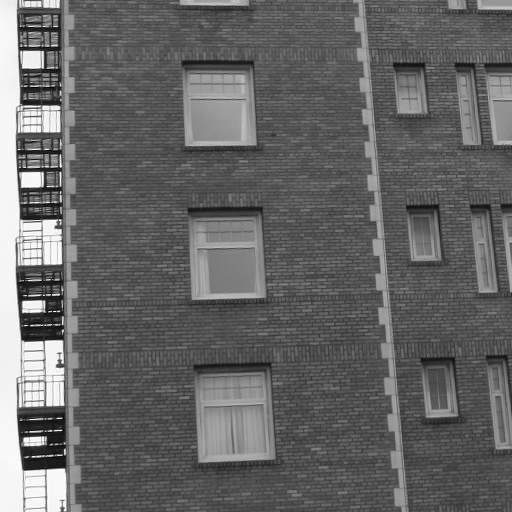
\includegraphics[width=5cm]{../LAB2/img/bricks_bw.png}
    \includegraphics[width=5cm]{../LAB2/output/2_3_downscaled_no_filter_bricks_bw.png} \\
    \includegraphics[width=5cm]{../LAB2/output/2_3_gauss_4_bricks_bw.png}
    \includegraphics[width=5cm]{../LAB2/output/2_3_gauss_8_bricks_bw.png}
    \caption{Top: Original image, image downsampled without anti-aliasing. \\ Bottom: Downsampled and gaussian filter with $\sigma = 0.4$ and $\sigma = 0.8$}
    \label{gaussian_anti_aliasing_filter_results}
\end{figure}

\newpage
\subsection*{2.4 - Derivative filters}

See listing \ref{gradient_task} for implementation details. Figure \ref{gradient_magnitude_image} shows the gradient magnitude image, and figure \ref{gradient_vector_field_image} shows the original image with the gradient vector field superimposed.

\begin{lstlisting}[language=Python, label=gradient_task, caption=Gradient]
import matplotlib.pyplot as plt
from numpy import gradient
from scipy.ndimage import gaussian_gradient_magnitude


def task2_4():
    img = normalize_intensity(imread(CAMERAMAN))
    img = img[30:95, [i for i in range(80, 160)]]  # select subsection of image
    vel_x, vel_y = gradient(f=img)

    magn_img = gaussian_gradient_magnitude(img, 3)
    output_path = os.path.join(OUTPUT_DIR, "2_4_gradien_magnitude_" + os.path.split(CAMERAMAN)[-1])
    imsave(output_path, magn_img)

    dim_x, dim_y = len(img[0]), len(img)
    x, y = range(dim_x), range(dim_y)
    x, y = meshgrid(x, y)
    plt.figure()
    imgplot = plt.imshow(img)
    imgplot.set_cmap('gray')
    plt.ylim(dim_y, 0)
    plt.quiver(x, y, vel_x, vel_y, pivot='middle')
    plt.show()
\end{lstlisting}

\begin{figure}[h!]
    \centering
    \includegraphics[width=5cm]{../LAB2/output/2_4_gradien_magnitude_cameraman.png}
    \caption{Gradient magnitude image}
    \label{gradient_magnitude_image}
\end{figure}

\newpage
\begin{figure}[h!]
    \centering
    \includegraphics[width=\linewidth]{../LAB2/output/2_4_vector_field_cameraman.png}
    \caption{Gradient vector field superimposed on original image}
    \label{gradient_vector_field_image}
\end{figure}

\newpage
\section*{Task 3 - Frequency Domain Filtering}

\subsection*{3.1 - Fourier Transform}

See listing \ref{fourier_spectrum} for implementation, figure \ref{fft_spectrum_image} for spectrum images.

\begin{lstlisting}[language=Python, label=fourier_spectrum, caption=Fourier transform and spectrum image]
from numpy.fft import fft2, fftshift


def task3_1():
    print('3.1')
    c_img = normalize_intensity(imread(CAMERAMAN))
    fft_res = fft2(a=c_img)
    output_path = os.path.join(OUTPUT_DIR, "3_1_fft_spectrum_" + os.path.split(CAMERAMAN)[-1])
    imsave(output_path, log(1 + abs(fftshift(fft_res))))

    b_img = normalize_intensity(imread(BRICKS))
    fft_res = fft2(a=b_img)
    output_path = os.path.join(OUTPUT_DIR, "3_1_fft_spectrum_" + os.path.split(BRICKS)[-1])
    imsave(output_path, log(1 + abs(fftshift(fft_res))))
\end{lstlisting}

\begin{figure}[h!]
    \centering
    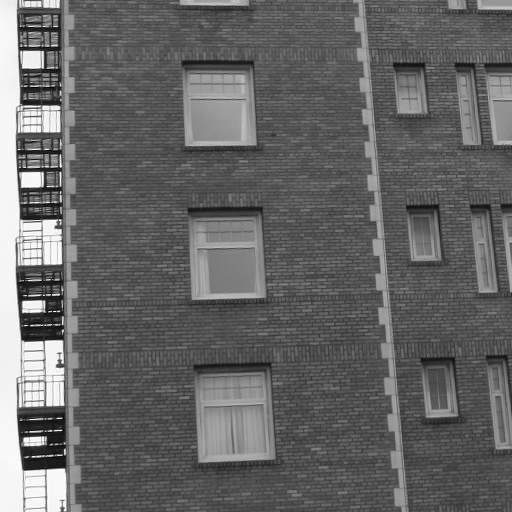
\includegraphics[width=5cm]{../LAB2/img/bricks_bw.png}
    \includegraphics[width=5cm]{../LAB2/output/3_1_fft_spectrum_bricks_bw.png} \\
    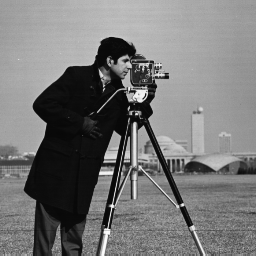
\includegraphics[width=5cm]{../LAB2/img/cameraman.png}
    \includegraphics[width=5cm]{../LAB2/output/3_1_fft_spectrum_cameraman.png}
    \caption{Original on the left, corresponding spectrum on the right.}
    \label{fft_spectrum_image}
\end{figure}

\newpage
\subsection*{3.2 - Low- and High-pass}

See listing \ref{lo_hi_pass} for implementation. Figure \ref{lo_hi_pass_figure} shows the results.

\begin{lstlisting}[language=Python, label=lo_hi_pass, caption=Fourier transform and spectrum image]
def task3_2():
    print('3.2')
    low_pass = normalize_intensity(imread(LOW_PASS))
    high_pass = normalize_intensity(imread(HIGH_PASS))

    img_freq_dom = fft2(a=normalize_intensity(imread(BRICKS_2)))
    apply_low_pass = img_freq_dom * low_pass
    ifft_res = ifft2(a=apply_low_pass)
    output_path = os.path.join(OUTPUT_DIR, "3_2_low_pass_" + os.path.split(BRICKS_2)[-1])
    imsave(output_path, abs(ifft_res))

    apply_high_pass = img_freq_dom * high_pass
    ifft_res = ifft2(a=apply_high_pass)
    output_path = os.path.join(OUTPUT_DIR, "3_2_high_pass_" + os.path.split(BRICKS_2)[-1])
    imsave(output_path, abs(ifft_res))
\end{lstlisting}

\begin{figure}[h!]
    \centering
    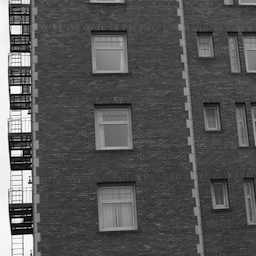
\includegraphics[width=5cm]{../LAB2/img/bricks_bw_256.png}
    \includegraphics[width=5cm]{../LAB2/output/3_2_high_pass_bricks_bw_256.png}
    \includegraphics[width=5cm]{../LAB2/output/3_2_low_pass_bricks_bw_256.png}
    \caption{Original image, high-pass filter applied, low-pass filter applied.}
    \label{lo_hi_pass_figure}
\end{figure}
